%%%%%%%%%%%%%%%%%%%%%%%%%%%%%%%%%%%%%%%%%%%%%%%%%%%%%%%%%%%%%%%%%%%%%%%%%%%%%%%%
% Template for USENIX papers.
%
% History:
%
% - TEMPLATE for Usenix papers, specifically to meet requirements of
%   USENIX '05. originally a template for producing IEEE-format
%   articles using LaTeX. written by Matthew Ward, CS Department,
%   Worcester Polytechnic Institute. adapted by David Beazley for his
%   excellent SWIG paper in Proceedings, Tcl 96. turned into a
%   smartass generic template by De Clarke, with thanks to both the
%   above pioneers. Use at your own risk. Complaints to /dev/null.
%   Make it two column with no page numbering, default is 10 point.
%
% - Munged by Fred Douglis <douglis@research.att.com> 10/97 to
%   separate the .sty file from the LaTeX source template, so that
%   people can more easily include the .sty file into an existing
%   document. Also changed to more closely follow the style guidelines
%   as represented by the Word sample file.
%
% - Note that since 2010, USENIX does not require endnotes. If you
%   want foot of page notes, don't include the endnotes package in the
%   usepackage command, below.
% - This version uses the latex2e styles, not the very ancient 2.09
%   stuff.
%
% - Updated July 2018: Text block size changed from 6.5" to 7"
%
% - Updated Dec 2018 for ATC'19:
%
%   * Revised text to pass HotCRP's auto-formatting check, with
%     hotcrp.settings.submission_form.body_font_size=10pt, and
%     hotcrp.settings.submission_form.line_height=12pt
%
%   * Switched from \endnote-s to \footnote-s to match Usenix's policy.
%
%   * \section* => \begin{abstract} ... \end{abstract}
%
%   * Make template self-contained in terms of bibtex entires, to allow
%     this file to be compiled. (And changing refs style to 'plain'.)
%
%   * Make template self-contained in terms of figures, to
%     allow this file to be compiled. 
%
%   * Added packages for hyperref, embedding fonts, and improving
%     appearance.
%   
%   * Removed outdated text.
%
%%%%%%%%%%%%%%%%%%%%%%%%%%%%%%%%%%%%%%%%%%%%%%%%%%%%%%%%%%%%%%%%%%%%%%%%%%%%%%%%

\documentclass[letterpaper,twocolumn,10pt]{article}
\usepackage{usenix-2020-09}

% to be able to draw some self-contained figs
\usepackage{tikz}
\usepackage{amsmath}

% inlined bib file
\usepackage{filecontents}

%-------------------------------------------------------------------------------
\begin{filecontents}{\jobname.bib}
%-------------------------------------------------------------------------------
@Book{arpachiDusseau18:osbook,
  author =       {Arpaci-Dusseau, Remzi H. and Arpaci-Dusseau Andrea C.},
  title =        {Operating Systems: Three Easy Pieces},
  publisher =    {Arpaci-Dusseau Books, LLC},
  year =         2015,
  edition =      {1.00},
  note =         {\url{http://pages.cs.wisc.edu/~remzi/OSTEP/}}
}
@InProceedings{waldspurger02,
  author =       {Waldspurger, Carl A.},
  title =        {Memory resource management in {VMware ESX} server},
  booktitle =    {USENIX Symposium on Operating System Design and
                  Implementation (OSDI)},
  year =         2002,
  pages =        {181--194},
  note =         {\url{https://www.usenix.org/legacy/event/osdi02/tech/waldspurger/waldspurger.pdf}}}
\end{filecontents}

%-------------------------------------------------------------------------------
\begin{document}
%-------------------------------------------------------------------------------

%don't want date printed
\date{}

% make title bold and 14 pt font (Latex default is non-bold, 16 pt)
\title{\Large \bf Research Proposal: \\Pruning Techniques for the Quanto Quantum Curcuit Optimizer}

%for single author (just remove % characters)
\author{
{\rm Max von Storch}\\
Technische Universität München
\and
{\rm Johannes Schielein}\\
Technische Universität München
% copy the following lines to add more authors
% \and
% {\rm Name}\\
%Name Institution
} % end author

\maketitle

%-------------------------------------------------------------------------------
\begin{abstract}
%-------------------------------------------------------------------------------
This report is about Quanto, a quantum circuit optimizers with uses automated circuit identity generation, and our approach to optimize
it by pruning the space of possible circuits.   
\end{abstract}


%-------------------------------------------------------------------------------
\section{Part A: Paper Summary}
%-------------------------------------------------------------------------------

\subsection{Context of the work (``Why?'')}
\begin{itemize}
  \item \textbf{What is the problem?}
  \item \textbf{Why is it important or interesting?}
  \item \textbf{What is the state-of-the-art? What is the “research gap”?}
  \item \textbf{Why is it difficult? Or what are the challenges?}
\end{itemize}

\subsection{Contributions of the work (``How?'')}
\begin{itemize}
  \item \textbf{What is the proposed solution?}
  \item \textbf{How it works at a high-level?}
  \item \textbf{What are the key insights?}
  \item \textbf{Or what are the novel aspects?}
\end{itemize}

%-------------------------------------------------------------------------------
\section{Research proposal: Pruning Methods}
%------------------------------------------------------------------------------
\subsection{Motivation}
As stated in the Quanto Paper the number of possible circuits grows exponentially with an increasing number of qubits and
increasing circuit depth. In our opinion this is the biggest limiting factor for this type of optimization since it limits the possibilities to optimize larger circuits.

The original method introduced tiling as a work around while this greatly improves the level of optimization for larger circuits it still doesn't provide the same
quality of optimization and also speed as a database of larger circuits would do. 

Another Problem is the size of the database itself.The proposed algorithm in the Quanto paper stores all possible circuit in its database not only the most optimal one. This adds a lot of redundancy to the database.

Pruning the search space of all possible quantum circuit is therefore crucial to improving the optimizer further. 

\subsection{Implications and Limitations}
One important change that comes to the structure of the optimizer is that the dictionary that maps the circuits to its fingerprint cant be created and used any more. This is due to the fact that due to pruning the search space we won't iterate over all circuits and therefore can't compute the mapping from circuits to fingerprints any more.

If we would create the dictionary in an additional step we could also group these circuits based on their equivalence with no significant increase in computation time, making the proposed pruning basically useless.\\

In our research we limited ourselves to optimizing the depth of the circuit as it was the primary optimization goal of the Quanto optimizer.

\subsection{Notations and Definitions}
Before going over our pruning technique some words on definitions and important terms that are used in the following sections.\\
We use the same notation for the \textbf{gate set}, \textbf{depth} and \textbf{qubit number}. 

Additionally we define $C$ or $C^1$ as the set of all circuits with $n$ qubits and a depth of one and $C^k$ as all Circuits of length $k$. The $[a]_\sim$ Operator returns all circuits that are equivalent to $a$.


 
\begin{description}
	\item[optimal] A quantum circuit is called optimal if there exists no equivalent circuit with lower cost
	
	\item[Column circuit] A circuit with maximum depth of one
\end{description}

For the concatenation of two circuits $a$ and $b$ with the same number of qubits we write $a\Vert b$


% -----------------------------------------------------------------------------------
\subsection{Challenges}
When we prune the search space of circuits we discard circuits we don't consider. When doing this we need to be careful that we still manage to reach all circuits 
(or equivalent circuits $[a]_\sim\space\forall a\in C^d$). The pruned database must also include all optimal circuits.

At the same time pruning adds overhead to the computation of the database. Se we need to make sure that the expense of these added computational steps don't exceed the advantages of the pruning.

Balancing these two aspects of cutting away enough to gain a net profit and leaving enough left to have all possibilities covered is a difficult task.

\subsection{Pruning Approach}
We started our research for pruning techniques by looking into the circuits of the Quanto database. A lot of the solutions in there are obviously not optimal or redundant: circuits including two \texttt{X} Gates concatenated or a column circuit only consisting of identity gates. 

Investigating further into these redundancies, we found that most of the time, these non optimal circuits were \textit{subcircuits} of larger structures. Replacing these subcircuits with an optimal equivalent, would greatly improve the cost of the total circuit. On the other hand appending column circuits to a not optimal circuit can't really result in an optimal one, so there is no need to further consider them in future iterations.\\

For each iteration we could generate new circuits and check for each of them if there already exists a less expensive circuit in the database if so we can discard the circuit. That would greatly reduce the number of possibilities to consider in the following iterations and limits the entries in the database to the most optimal ones.

\subsubsection{Proposed Algorithm}

The following code-segment shows a algorithm for generating the identity database with the described pruning approach:
\begin{verbatim}
function generateDatabase(n,d,gs){
	db = dict() 	# init database
	ws = dict() 	# init Working-Set
	ws[1] = generateColumns(n,gs)
	ws[1].remove([I,...,I]) 	# remove identity-c.
	
	for i in range(2,d) {
		for c in ws[i-1] {
			for r in ws[1] {
				c'=c||r
				if c' not in db {
					db[fingerprint(c')] = c'
					ws[i].add(c')
					continue
				}
				if isOptimal(c', db) {
					m = db[fingerprint(c')]
					db[fingerprint(c')] = c'	
					ws[i].add(c')
					ws[i].remove(m)
				}
	}}} 	# End for loops
} 	# End function
\end{verbatim}

The algorithm starts with initializing the database and working set dictionaries and generates all possible column circuits for \texttt{n} qubits and a gate-set using the \texttt{generateColumns(n,gs)}. It also removes the column circuit that only consists of identity gates.\\

Next, the program iterates over the depth levels starting with a depth of two. For each iteration we take each element from the working set of the previous round and append each column circuit to it. For each of these newly generated circuits the algorithm checks if there already exists an equivalent circuit in the database. 

If the circuit is completely new it gets added to the current working set and the database. 

If there exists an equivalent circuit we check if the new circuit has lower costs than the existing one, if so we replace it in the database and if applicable in the current working set. 

If there exists an optimal solution we don't add the new solution to the current working set.

The \texttt{isOptimal(c,db)} checks if \texttt{c} is optimal with regards to the current database \text{db} and returns a boolean respectively.\\

It follows from the definition of the algorithm that every element in $ws[i]\space\forall i$ is optimal. 

For every existing circuit with $n$ Qubits and depth $d$ there exists at lease an equivalent circuit in the pruned database. To show that we assume that there exists a circuit $a\Vert b$ of depth $j$ with $a\not\in ws[j-1]$. Then because of the definition of the algorithm we know that there must already exist an equivalent circuit in our database $a'$. From that it follows that $a'\Vert b\equiv a\Vert b$. Either $a'\Vert b$ is optimal and therefore in the database or there already exists an equivalent optimal circuit $c$ with $c\equiv a\Vert b$

\subsubsection{Evaluation}
The amount of the saving depends on the depth of the circuit and the number of qubits but also on the used gate set, which makes it hard to quantify. 

However we can say that for $S_l$ column circuits the removal of one circuit in the k-th iteration, results in $S_l^{d-k}$ less circuits the algorithm iterates over.\\

The size of the final database also greatly decreased since only optimal circuits are stored. This should also speed up the lookup in the optimization phase.
\subsection{Context of your research (``Why?'')}
\begin{itemize}
  \item \textbf{What is the problem?}
  \item \textbf{Why is it important or interesting?}
  \item \textbf{Why is it difficult? Or what are the challenges?}
\end{itemize}

\subsection{Approach of your research work (``How?'')}
\begin{itemize}
  \item \textbf{What is the proposed solution? How does it work?}
  \item \textbf{What are the key insights?}
  \item \textbf{Or what are the novel aspects?}
\end{itemize}

%-------------------------------------------------------------------------------
\section{Footnotes, Verbatim, and Citations}
%-------------------------------------------------------------------------------

Footnotes should be places after punctuation characters, without any
spaces between said characters and footnotes, like so.%
\footnote{Remember that USENIX format stopped using endnotes and is
  now using regular footnotes.} And some embedded literal code may
look as follows.

\begin{verbatim}
int main(int argc, char *argv[]) 
{
    return 0;
}
\end{verbatim}

Now we're going to cite somebody. Watch for the cite tag. Here it
comes. Arpachi-Dusseau and Arpachi-Dusseau co-authored an excellent OS
book, which is also really funny~\cite{arpachiDusseau18:osbook}, and
Waldspurger got into the SIGOPS hall-of-fame due to his seminal paper
about resource management in the ESX hypervisor~\cite{waldspurger02}.

The tilde character (\~{}) in the tex source means a non-breaking
space. This way, your reference will always be attached to the word
that preceded it, instead of going to the next line.

And the 'cite' package sorts your citations by their numerical order
of the corresponding references at the end of the paper, ridding you
from the need to notice that, e.g, ``Waldspurger'' appears after
``Arpachi-Dusseau'' when sorting references
alphabetically~\cite{waldspurger02,arpachiDusseau18:osbook}. 

It'd be nice and thoughtful of you to include a suitable link in each
and every bibtex entry that you use in your submission, to allow
reviewers (and other readers) to easily get to the cited work, as is
done in all entries found in the References section of this document.

Now we're going take a look at Section~\ref{sec:figs}, but not before
observing that refs to sections and citations and such are colored and
clickable in the PDF because of the packages we've included.

%-------------------------------------------------------------------------------
\section{Floating Figures and Lists}
\label{sec:figs}
%-------------------------------------------------------------------------------


%---------------------------
\begin{figure}
\begin{center}
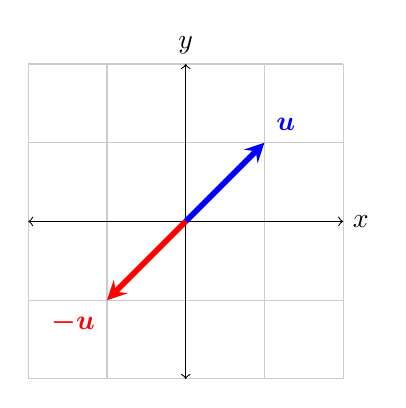
\begin{tikzpicture}
  \draw[thin,gray!40] (-2,-2) grid (2,2);
  \draw[<->] (-2,0)--(2,0) node[right]{$x$};
  \draw[<->] (0,-2)--(0,2) node[above]{$y$};
  \draw[line width=2pt,blue,-stealth](0,0)--(1,1)
        node[anchor=south west]{$\boldsymbol{u}$};
  \draw[line width=2pt,red,-stealth](0,0)--(-1,-1)
        node[anchor=north east]{$\boldsymbol{-u}$};
\end{tikzpicture}
\end{center}
\caption{\label{fig:vectors} Text size inside figure should be as big as
  caption's text. Text size inside figure should be as big as
  caption's text. Text size inside figure should be as big as
  caption's text. Text size inside figure should be as big as
  caption's text. Text size inside figure should be as big as
  caption's text. }
\end{figure}
%% %---------------------------


Here's a typical reference to a floating figure:
Figure~\ref{fig:vectors}. Floats should usually be placed where latex
wants then. Figure\ref{fig:vectors} is centered, and has a caption
that instructs you to make sure that the size of the text within the
figures that you use is as big as (or bigger than) the size of the
text in the caption of the figures. Please do. Really.

In our case, we've explicitly drawn the figure inlined in latex, to
allow this tex file to cleanly compile. But usually, your figures will
reside in some file.pdf, and you'd include them in your document
with, say, \textbackslash{}includegraphics.

Lists are sometimes quite handy. If you want to itemize things, feel
free:

\section{Research Proposal: Search Space Pruning}

\begin{description}
  
\item[fread] a function that reads from a \texttt{stream} into the
  array \texttt{ptr} at most \texttt{nobj} objects of size
  \texttt{size}, returning returns the number of objects read.

\item[Fred] a person's name, e.g., there once was a dude named Fred
  who separated usenix.sty from this file to allow for easy
  inclusion.
\end{description}

\noindent
The noindent at the start of this paragraph in its tex version makes
it clear that it's a continuation of the preceding paragraph, as
opposed to a new paragraph in its own right.


\subsection{LaTeX-ing Your TeX File}
%-----------------------------------

People often use \texttt{pdflatex} these days for creating pdf-s from
tex files via the shell. And \texttt{bibtex}, of course. Works for us.

%-------------------------------------------------------------------------------
\section*{Acknowledgments}
%-------------------------------------------------------------------------------

The USENIX latex style is old and very tired, which is why
there's no \textbackslash{}acks command for you to use when
acknowledging. Sorry.

%-------------------------------------------------------------------------------
\section*{Availability}
%-------------------------------------------------------------------------------

USENIX program committees give extra points to submissions that are
backed by artifacts that are publicly available. If you made your code
or data available, it's worth mentioning this fact in a dedicated
section.

%-------------------------------------------------------------------------------
\bibliographystyle{plain}
\bibliography{\jobname}

%%%%%%%%%%%%%%%%%%%%%%%%%%%%%%%%%%%%%%%%%%%%%%%%%%%%%%%%%%%%%%%%%%%%%%%%%%%%%%%%
\end{document}
%%%%%%%%%%%%%%%%%%%%%%%%%%%%%%%%%%%%%%%%%%%%%%%%%%%%%%%%%%%%%%%%%%%%%%%%%%%%%%%%

%%  LocalWords:  endnotes includegraphics fread ptr nobj noindent
%%  LocalWords:  pdflatex acks
